\pagebreak
\checkoddpage
\ifodd\thepage
	\null
	\newpage
\fi

\setcounter{chapter}{4} % Manually set the chapter counter to 4, so that the figure below will receive a chapter numbering of 4
\setcounter{figure}{0}  % Reset the figure counter to 0 so that this figure will be the first figure in chapter 3
\thispagestyle{empty}

\begin{minipage}{\textwidth}
	\vspace{2.25cm}
	{%
		\centering
		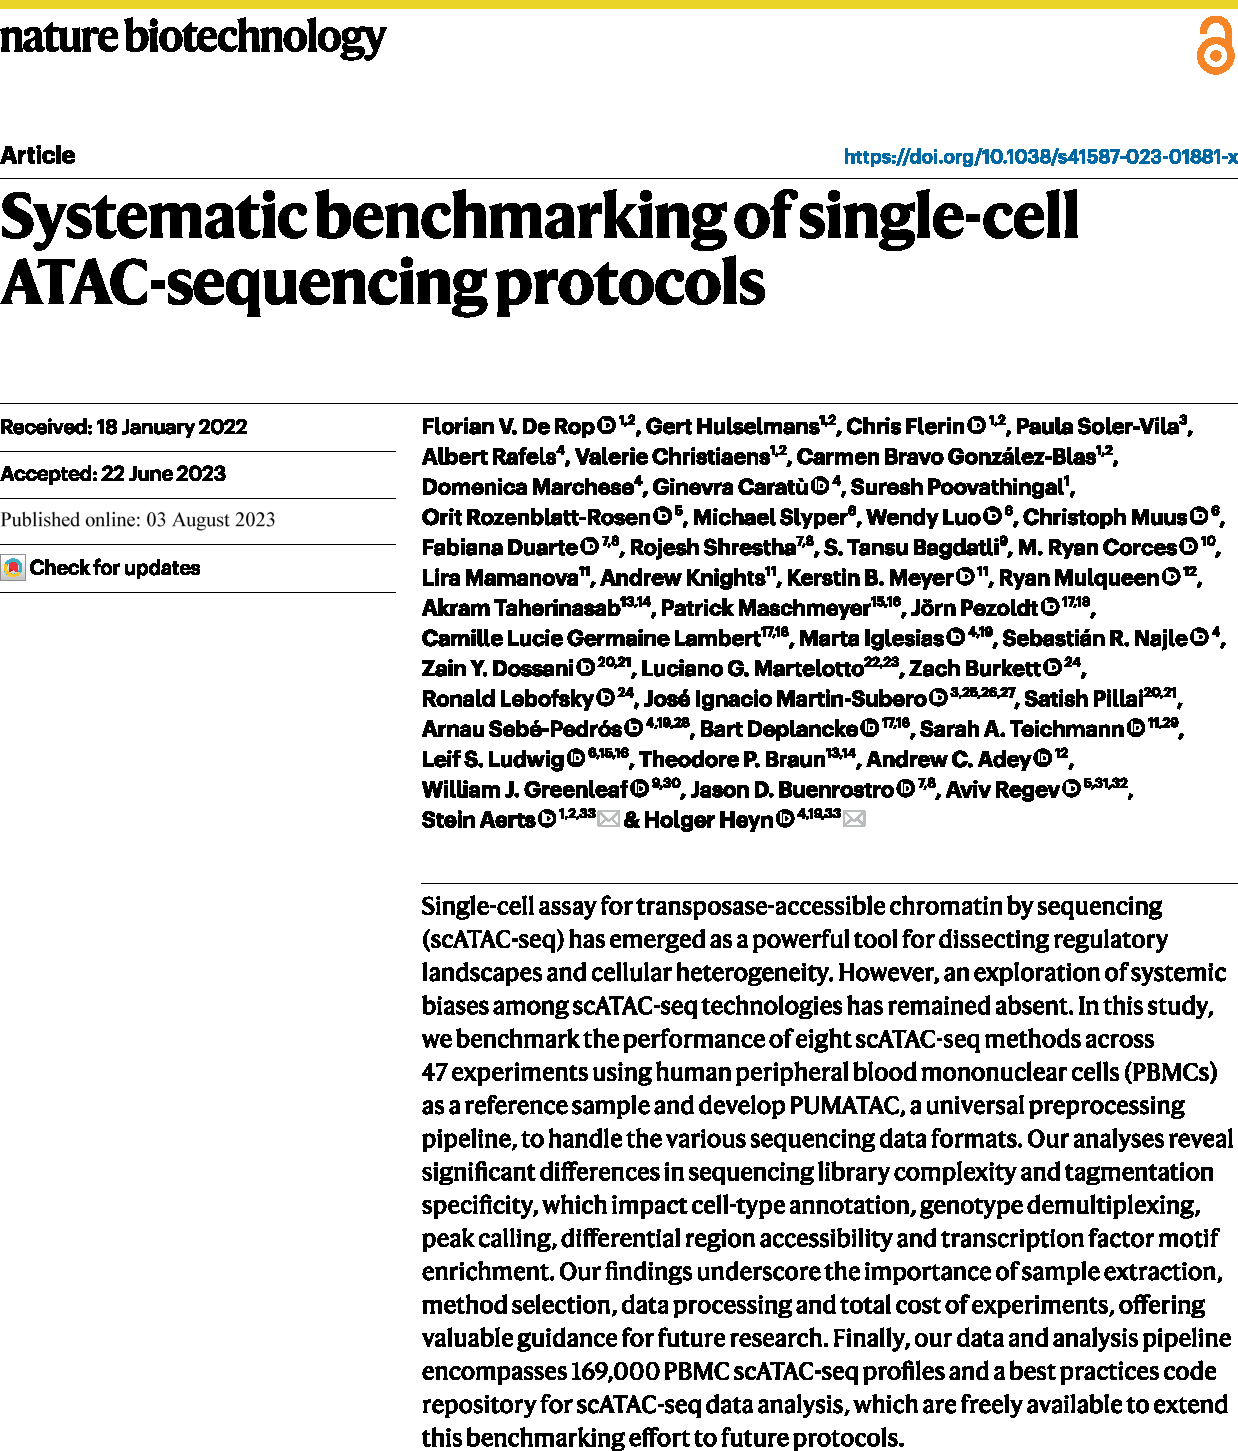
\includegraphics[width=\textwidth]{im/2023_nbt_fixed.pdf}
		\captionsetup{width=0.80\linewidth}
		\vspace{0.5cm}
		\captionof{figure}[Article title page of "Systematic benchmarking of single-cell ATAC sequencing protocols"]{Article title page of "Systematic benchmarking of single-cell ATAC sequencing protocols"}
		\label{fig:article_title_benchmark}
	}%
\end{minipage}
% \setcounter{chapter}{3} % Manually reset the chapter counter to 3

\chapter{Benchmarking the performance of single-cell chromatin accessibility sequencing methods}
\setcounter{figure}{1}  % Set the figure counter to 1 already to include the first figure
The following chapter will describe how we benchmarked several of the most prominent scATAC-seq techniques available in 2023. We performed 47 experiments across 8 different scATAC-seq methods to generate 169k single-cell chromatin accessibility profiles. Our benchmark quantified reproducible technical biases in not only the sensitivity, but also the specificity of these methods, produced a scATAC-seq pre-processing pipeline with best practices tutorials, and yielded the largest dataset of scATAC-seq in PBMCs to date. This work was published in \fullcite{deropSystematicBenchmarkingSinglecell2023} (\autoref{fig:article_title_benchmark}).

\section{Motivation and approach}
Throughout the development of HyDrop-ATAC, we were often confronted with questions surrounding the method's sensitivity (the number of fragments detected per cell) and specificity (the enrichment of these fragments in enhancers and near transcription start sites, collectively forming chromatin accessibility "peaks"). Such questions arose both internally and externally, and echoed previous calls for an in-depth method performance exploration since the release of Bio-Rad\supershortnotecite{lareauDropletbasedCombinatorialIndexing2019} and 10x Genomics'\supershortnotecite{satpathyMassivelyParallelSinglecell2019} scATAC-seq products in 2019. At the time, a number of open-source scATAC-seq protocols had also been published\sjcitep[,]{chenRapidRobustMethod2018,mulqueenHighcontentSinglecellCombinatorial2021} [sci, name each of these techniques individually with ref, also mulqueen was not published yet!], but best-case data exhibited in these articles revealed that they could not compete with 10x in terms of sensitivity. Furthermore, most of these open-source protocols required significant levels of expertise (e.g. low-level automated liquid handling) and/or non-commercially available components (e.g. indexed Tn5). As a result, they remained in use almost exclusively at a handful of labs. Both BioRad and 10x's scATAC-seq solutions were more user-friendly and handled the most technically challenging aspect, microfluidic droplet generation, on benchtop devices (10x's Chromium Controller and Bio-Rad's ddSEQ). However, the Chromium controller was already ubiquitously present in our research due to the success of 10x's scRNA-seq products. As a result, 10x enjoyed a relatively competition-free dominance of the scATAC-seq market, leading to [x] publications compared to ddSEQ's [y], and only approximately [z] publications generated with open-source methods by [date].

We reasoned that an exact quantification of the performance differences among commercial and non-commercial protocols could stimulate informed decision making. Two such benchmarks had been performed for scRNA-seq methods: one by Ziegenhain and Enard\sjcitep[,]{ziegenhainComparativeAnalysisSingleCell2017} and a larger, more recent study by Mereu and Heyn\sjcitep[.]{mereuBenchmarkingSinglecellRNAsequencing2020} Both of these benchmarks employed the same strategy: a reference sample was distributed to collaborating labs [doublecheck for Ziegenhain], which each generated at least one scRNA-seq dataset. In the Mereu benchmark, the reference consisted of a mixture of [x] tissues across [y] species. This complicated genome alignment and further post-processing, and we therefore opted to limit the reference sample to a mixture of PBMC extracted from one male and one female donor. The use of a liquid tissue also simplified sample handling: PBMC can be distributed frozen, and only need to be thawed slowly before nuclei extraction can occur. In addition, a large reference dataset of single-cell PBMC chromatin accessibility did not yet exist.

We included 7 different techniques in the initial phase of our benchmark. [ref to introduction] includes an overview of these methods from a mechanistic point of view.:

\begin{itemize}[noitemsep]
	\item 10x Genomics scATAC-seq v1 and v1.1: The most widely used scATAC-seq method. While v1 reagent kits were technically still available for purchase, the microfluidic chip required for this kit had been decomissioned due to patent infringement litigation by BioRad [doublecheck this. was the v1 hard-linked to the v1 chip? could it be run on nextgem?]. An updated version (v1.1) was released together with the nextGEM chip, which circumvented the BioRad intellectual property by generating droplets in a reservoir deposition style instead of using flow focusing (fig?).
	\item 10x Multiome [check full name]: Introduced in [year], the 10x multiome kit generated both scRNA-seq and scATAC-seq data from the same cells. This novelty had previously only been demonstrated in plates [ref, doublecheck - when was scCAT-seq?]
	\item Bio-Rad ddSEQ SureCell ATAC: 10x's direct competitor. The Bio-Rad scATAC-seq method also used droplet microfluidics, but employed hard resin beads (like Drop-seq)\supershortnotecite{macoskoHighlyParallelGenomewide2015} and a ingenious overloading strategy to reach cell capture rates on par with 10x [ref introduction ddSEQ].
	\item mtscATAC-seq: A modification on the 10x protocol where omission of certain detergents during nuclei extraction keeps the cell membrane remain intact but permeabilized to Tn5. As a result, the cell's mitochondria are retained, and their genomes is also sequenced, allowing lineage tracing.
	\item s3-ATAC: The most sensitive combinatorial indexing/plate-based assay to date. s3-ATAC uses uracil-intolerant polymerases to terminate extension on the [x] chain. , circumventing the traditional 50\% loss in sensitivity due to homotypic-ended fragments [is there a ref that describes this problem?].
	\item HyDrop: Our own in-house method. HyDrop's workflow is very similar to 10x scATAC-seq, but uses commercially available reagents and the Onyx microfluidics controller in combination with an open-source chip to encapsulate cells.
\end{itemize}

Several other techniques were considered, but not included for various reasons:

\begin{itemize}[noitemsep]
	\item Fluidigm C1 scATAC-seq: This was the first commercially available scATAC-seq method.
	\item Chen \& Teichmann protocol: The first open-source scATAC-seq method. This method used up-front bulk tagmentation followed by FAC sorting into individual wells where accessible chromatin fragments from each cell were amplified separately [check this]
	\item sci-ATAC: Plans were made to include sci-ATAC, but due to practical reasons and limited labour bandwidth at competent labs, these were aborted. We sought to represent combinatorial indexing methods with s3-ATAC instead.
	\item dscCAT-seq: A resin-bead based microfluidic method for both ATAC- and RNA-seq from the same single cell - while this method was very innovative, relatively low sensitivity in both RNA and ATAC coupled with the difficulty of performing Drop-seq/DrONC-seq [check dronc] precluded its inclusion.
	\item ISSAAC-seq \& SHARE-seq: two additional scRNA + scATAC-seq combination methods, one droplet-based and the other combinatorial indexing based. both of these methods were published [late?]
\end{itemize}

Initially, [x] institutes were agreed to be part of the benchmarking effort ([list]), and generated a total of 16 datasets across these 7 protocols. In first revisions, reviewers unanimously agreed that we had too few replicates to draw significant conclusions from these datasets. Moreover, 10x Genomics had just released a version 2 of their scATAC-seq method, promising a 50\% increase in sensitivity. We decided to include this method and generate more technical replicates on the initial 7 techniques, yielding a total of 47 individual scATAC-seq datasets across 8 methods (\autoref{fig:scatac_seq_benchmark_study_final_datasets}). Each dataset was sequenced to sufficient depth, deposited centrally, and analysed at VIB.

	{%
		\centering
		\includegraphics[width=0.85\textwidth,height=5cm]{example-image-a}
		\captionsetup{width=0.80\linewidth}
		\captionof{figure}[scATAC-seq benchmark study final datasets]{scATAC-seq benchmark study final datasets}
		\label{fig:scatac_seq_benchmark_study_final_datasets}
	}%

\section{Analysis}
Early on in the project, we foresaw that data stemming from the 8 different techniques would strongly differ in sequencing format. The 10x Genomics format set the standard, each fragment yielding two paired-end genomic reads, a sample index read, and a 16 basepair barcode read matching a whitelist containing ~2.7M entries. HyDrop was designed with a similar structure in mind, but with a barcode length of 50 bp. Bio-Rad and s3-ATAC used a very different logic: [] (\autoref{fig:library_types_and_sequencing_schematics}).

	{%
		\centering
		\includegraphics[width=0.85\textwidth,height=8cm]{example-image-a}
		\captionsetup{width=0.80\linewidth}
		\captionof{figure}[Library types and sequencing schematics]{Library types and sequencing schematics}
		\label{fig:library_types_and_sequencing_schematics}
	}%

Moreover, among the several method-specific data analysis pipelines, there was no consensus as to how this data should be pre-processed and aligned to the reference genome. [short description of the different pipelines used, maybe keep low-level here and expand on cistopic/snapatac/archr,... later and show that cistopic consistently performs well]. We had faced a similar problem during the development of HyDrop: despite the structural similarities between 10x Genomics' and HyDrop's sequencing format, 10x's CellRanger software could not be used to pre-process HyDrop data since several internal parameters (such as read lengths and barcode whitelist) were hard-coded to match 10x data. To solve this problem, Gert Hulselmans and Christopher Flerin developed a NextFlow [di tomasso et al] pre-processing pipeline capable of aligning sequencing data agnostic of sequencing format (\autoref{fig:pumatac_workflow}).

	{%
		\centering
		\includegraphics[width=5cm,height=5cm]{example-image-a}
		\captionsetup{width=0.80\linewidth}
		\captionof{figure}[PUMATAC steps]{PUMATAC steps}
		\label{fig:pumatac_steps}
	}%

	[explanation of how PUMATAC works]

The use of NextFlow provides several advantages over shell scripts:

\begin{enumerate}[noitemsep]
	\item Intelligent interruption procedures: per step in the pipeline, an [md5] hash of the sample names, input files, output files and parameters is computed. If the workflow is interrupted and re-started, these hashes are re-computed. If no change in the hash is detected, no conditions have changed, and the pipeline can resume where it left off. If a parameter is changed, the hash of relevant steps will change, and the pipeline will resume there.
	\item Management of parallel processing: samples and steps that are not dependent on each other can be scheduled independently from each other's completion status, facilitating co-processing of small and large datasets. Each step in the pipeline has definitions for maximum CPU and memory usage, and available resources are utilised maximally.
	\item Built-in support for software containers (docker, singularity), improving environment-independent compatibility.
\end{enumerate}

Due to the large scale and collaborative nature of the project, sequencing data trickled in on an unpredictable basis.

	{%
		\centering
		\includegraphics[width=5cm,height=5cm]{example-image-a}
		\captionsetup{width=0.80\linewidth}
		\captionof{figure}[Data analysis workflow]{Data analysis workflow}
		\label{fig:data_analysis_workflow}
	}%


\section{Key results}
One of the most surprising findings of the benchmark was the comparison between different sources of data "loss" among different methods. While analysing data for unrelated projects, I noticed that in a given dataset, only a very small fraction of all sequenced reads ends up being "useful". For example, if a single-cell library of 10 000 cells is sequenced to 400 million reads total, and the resulting median number of unique fragments per cell in the count matrix is 5 000, then only 50 million reads are really used - a mere 12.5\% of the total. One of the most significant losses occurred during the "cell filtration" step. 


\section{Conclusions}

\lipsum[1]